
%!TEX program = xelatex
\documentclass[letterpaper,12pt]{exam}
\usepackage{../videoNotes}
\usepackage{xcolor}
\usepackage[dvipsnames]{xcolor}
\usepackage{soul}
\newcommand{\unit}{Unit 06}

\usepackage{draftwatermark}
\SetWatermarkText{DRAFT}
\SetWatermarkScale{1.5}
\SetWatermarkColor{red!20}

\pagestyle{headandfoot}
\firstpageheader{CSC 264 \semester\ \  \unit}{}{Name: $\rule{6cm}{0.15mm}$}
\runningheader{CSC 264 \semester}{\unit}{Page \thepage\ of \numpages}
\firstpagefooter{}{}{}
\runningfooter{}{}{}

\begin{document}

%\underconstruction

\section*{\unit\_005 -- Syntax}
\par{\fontfamily{qzc}\selectfont\textbf{Video Length 12:45}}
\begin{questions}

\begin{samepage}
    \question What is the difference between .ascii and the .asciz directive?
    \vspace{5mm}
\end{samepage}
\begin{samepage}
    \question How many bytes would the directive \textbf{\texttt{.ascii "dog"}} allocate?
    \vspace{5mm}
\end{samepage}
\begin{samepage}
    \question How many bytes would the directive \textbf{\texttt{.asciz "dog"}} allocate?
    \vspace{5mm}
\end{samepage}
\par
\begin{samepage}
    \question The code below declares a string.  Write the declaration of \texttt{len} that has the assembler calculate the length of message.
    \begin{verbatim}
         message: .ascii "Hello, World!"
         len:     .quad   
    \end{verbatim}        
    \vspace{5mm}
\end{samepage}
\par
 \begin{samepage}
     \question Modify the code below to load the address of message into the rdi register.
        \begin{verbatim}
            movq  letters, %rdi
        \end{verbatim}
     \vspace{5mm}
 \end{samepage}
 \par
 \begin{samepage}
     \question Modify the code below to load the contents of rdi into the r8b register.
        \begin{verbatim}
            movb  %rdi , %r8b
        \end{verbatim}
     \vspace{5mm}
 \end{samepage}
 \par 
 \question Consider the previous two questions.  One of them was moving a quad.  The second was only moving a byte.  Explain why.
\vspace{5mm}
 %----------------------------------

\section*{\unit\_010 -- Syscall}
\par{\fontfamily{qzc}\selectfont\textbf{Video Length 11:30}}
\begin{samepage}
    \question What is syscall?  Why do we need it?
    \vspace{5mm}
\end{samepage}
\par
\begin{samepage}
    \question Suppose you wanted to convert a program written for x86-64 to run on an ARM processor.  Would syscall need to be adapted to run on ARM?
    \vspace{5mm}
\end{samepage}
\par
 \begin{samepage}
     \question What three registers will we be using to communicate with syscall?
     \vspace{5mm}
 \end{samepage}
 \par
 \begin{samepage}
     \question If syscall is considered a function call, how are parameters passed to the function?
     \vspace{5mm}
 \end{samepage}
 \par
   
\rule{0.5\textwidth}{.4pt} %End of section
%----------------------------------
\section*{\unit\_020 Writing known length -- }
\par{\fontfamily{qzc}\selectfont\textbf{Video Length 14:00}}
\begin{samepage}
    \question What four registers are used for writing through the use of syscall?  What goes in each register? (You may refer to the cheatsheet for Exam 02)
    \begin{enumerate}
        \item 
        \vspace{5mm}
        \item 
        \vspace{5mm}
        \item 
        \vspace{5mm}
        \item 
        \vspace{5mm}
    \end{enumerate}
    \vspace{5mm}
\end{samepage}
\par

NOTE:  In the video I forgot to mention the return value in RAX.  After syscall, RAX contains the number of bytes written.
\begin{samepage}
    \question Write the 5 lines of code needed to print the string buffer named \textbf{\texttt{message}}.  There is no variable with the length, but you know it will always be 30 bytes long.
    \vspace{55mm}
\end{samepage}
\par
\rule{0.5\textwidth}{.4pt} %End of section
%----------------------------------
\section*{\unit\_030 -- Writing null-terminated strings, Part 1}
\par{\fontfamily{qzc}\selectfont\textbf{Video Length 13:45}}
\begin{samepage}
    \question Summarize in words (not in code) how to write a null terminated string if the length is not known in advance.
    \vspace{45mm}
\end{samepage}
\par
\begin{samepage}
    \question This was not discussed in the video.  Look closely at the code in the body of the loop.  Could any of the instructions done in the body of the loop have been done before the loop began?
    \vspace{5mm}
\end{samepage}
\par
 
\rule{0.5\textwidth}{.4pt} %End of section
%----------------------------------
\section*{\unit\_030 -- Optimized loop, part 2}
\par{\fontfamily{qzc}\selectfont\textbf{Video Length 9:30}}
\begin{samepage}
    \question Explain, in words, how the loop can be made to run faster.
    \vspace{35mm}
\end{samepage}
\par
\begin{samepage}
    \question This is asking for your opinion.  Am I being paranoid by putting the "movq \$1, \%rax" statement in the loop?  Explain your answer.
    \vspace{25mm}
\end{samepage}
\par
 \begin{samepage}
     \question Write out the loop by hand.  Think about it as you write it.  Did I miss any other improvements?  If so, comment on them. (The instructor is old school, and he still thinks that writing things by hand helps you understand them.)  Also, remember that the source code is on github in the sources folder if don't want to stare at the paused video to get the code.
     \vspace{75mm}
 \end{samepage}
 \par
  
\rule{0.5\textwidth}{.4pt} %End of section
%----------------------------------





\end{questions} 
%footer
\begin{center}
    \rule{0.667\textwidth}{.8pt} %End of section
\end{center}


If you have any lingering questions or problems, please write them here or see me.
\vfill
\begin{center}
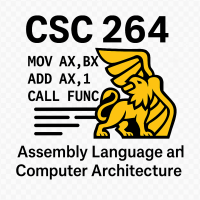
\includegraphics{../csc264Logo}
\end{center}
\end{document} 